\chapter{Background}

\textit{Give a background on basketball, sports predictions in general, sports predictions on basketball and theoretical concepts used in the report.}

\section{Basketball}
Basketball is a popular sport played by teams with 5 players on each side.  Seasons are played across two years, beginning in October and ending in April of the following year.  For the purposes of this paper, when a season is discussed for example the 2016 season, it will be in reference to the 2015-16 season.

There are 5 players on court per team, each with their own responsibilities summarized below by position \cite{player_criteria}:

\begin{itemize}
	\item \textbf{Point Guard:} They are the play maker, the ball is usually in their hands.  They organize the team's play and control the intensity of play.
	\item \textbf{Shooting Guard:}
	\item \textbf{Small Forward:}
	\item \textbf{Power Forward:}
	\item \textbf{Centre:}
\end{itemize}

\section{Theoretical Concepts}

\subsection{Poisson Distribution}
The Poisson distribution is defined by the formula \cite{poisson}

\begin{equation}
p_x(\lambda) = \frac{e^{-\lambda}\lambda^x}{x!}
\end{equation}

Figure \ref{fig:poisson} shows the probability mass function for the Poisson distribution with various $\lambda$.  The $y$ axis is the probability of $k$ occurring given the mean $\lambda$.  \textit{Cite This ->} The function is only defined at integer values of $k$.

\begin{figure}[!htb]
	\centering
	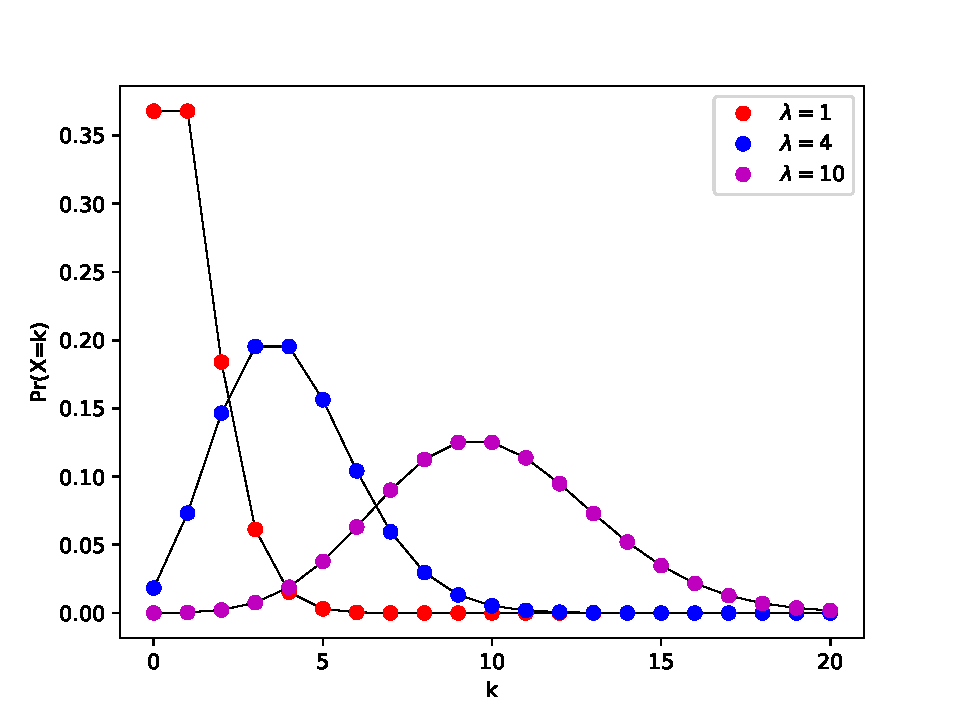
\includegraphics[width=0.75\textwidth]{{Figures/poisson_dist.pdf}}
	\captionof{figure}{Probability mass function of the Poisson Distribution}
	\label{fig:poisson}
\end{figure}

\subsection{Beta Distribution}

The Beta distribution is to assess probabilities.